% Created 2021-11-07 Sun 15:31
% Intended LaTeX compiler: pdflatex
\documentclass[presentation]{beamer}
\usepackage[utf8x]{inputenc}
\usepackage[T1]{fontenc}
\usepackage{graphicx}
\usepackage{grffile}
\usepackage{longtable}
\usepackage{wrapfig}
\usepackage{rotating}
\usepackage[normalem]{ulem}
\usepackage{amsmath}
\usepackage{textcomp}
\usepackage{amssymb}
\usepackage{capt-of}
\usepackage{hyperref}
\usetheme[height=20pt]{Rochester}
\author{Shane Mulligan \\  }
\date{\textit{<2021-03-01 Mon>}}
\title{EmacsConf 2021\ldots{} \\   \emph{\alert{Imaginary Programming with Emacs}} \\  }
\hypersetup{
 pdfauthor={Shane Mulligan \\  },
 pdftitle={EmacsConf 2021\ldots{} \\   \emph{\alert{Imaginary Programming with Emacs}} \\  },
 pdfkeywords={},
 pdfsubject={University of Otago},
 pdfcreator={Emacs 28.0.50 (Org mode 9.3.6)}, 
 pdflang={English}}
\begin{document}

\maketitle

\section{Presentation}
\label{sec:org71cb605}
\begin{frame}[label={sec:org85029f6}]{Following along}
\begin{block}{Repositories for following along}
{\tiny
\begin{center}
\begin{tabular}{l}
\url{http://github1s.com/semiosis/pen.el}\\
\url{http://github1s.com/semiosis/prompts}\\
\url{https://mullikine.github.io/posts/imaginary-programming-with-gpt-3/}\\
\href{http://github.com/semiosis/glossaries-gh/blob/master/imaginary-programming.txt}{imaginary programming glossary}\\
\href{http://github.com/semiosis/glossaries-gh/blob/master/imaginary-computing.txt}{imaginary computing glossary}\\
\href{http://github.com/semiosis/glossaries-gh/blob/master/semiosis-protocol.txt}{semiosis protocol glossary}\\
\href{http://github.com/semiosis/glossaries-gh/blob/master/pen.el.txt}{Pen.el glossary}\\
\href{https://arxiv.org/abs/2107.13586}{https://arxiv.org/abs/2107.13586 Pre-train, Prompt, and Predict}\\
\href{http://github1s.com/mullikine/imaginary-programming-transcript-emacsconf-2021}{talk transcript}\\
\end{tabular}
\end{center}
}
\end{block}
\end{frame}

\section{Imaginary Programming (IP) with Emacs}
\label{sec:orge076846}
\begin{frame}[label={sec:org20e4568},fragile]{Imaginary Programming (IP) (EmacsConf 2021)}
 \begin{block}{Objectives}
\begin{itemize}
\item Explain \texttt{Imaginary Computing}
\begin{itemize}
\item AI imagination
\item Discussing AI-generated artwork with an AI
\item Intelligent NFTs
\item Imaginary Web
\begin{itemize}
\item Paracosm vs Metaverse
\end{itemize}
\end{itemize}
\item Explain the \texttt{Philosophy} of IP
\begin{itemize}
\item Simulacra and Science Fiction
\item Truth (epistemology and alethiology)
\item Structuralism: Language based on sign relations
\end{itemize}
\item \texttt{Demo} Imaginary Programming
\begin{itemize}
\item Demonstrate \texttt{ilambda.el}
\end{itemize}
\end{itemize}
\end{block}
\end{frame}

\section{Imaginary Computing}
\label{sec:org40577a1}
\begin{frame}[label={sec:orgc4b7658}]{Imaginary Computing: AI Imagination}
\begin{block}{Language Models is programming for AIs}
LMs are our best friends in the AI model
menagerie because they make things
intelligible -- by understanding our textual
languages.
\end{block}

\begin{block}{Research}
\begin{itemize}
\item \href{https://www.youtube.com/watch?v=d-bvsJWmqlc}{Demis Hassabis: creativity and AI}
\end{itemize}
\end{block}
\end{frame}

\section{Imaginary Computing}
\label{sec:org2ad6e2a}
\begin{frame}[label={sec:orgd9507f5},fragile]{Imaginary Computing: Emacs as the shell}
 \begin{block}{Example: AI Art described by AI}
I use AlephAlpha’s multimodal LM to generate
\texttt{Alt text} for the eww web browser. This is in
order to keep websites textual.

\begin{itemize}
\item \href{https://mullikine.github.io/posts/alephalpha-for-alttext/}{AlephAlpha for alttext; Browsing the paracosm}
\item \href{https://mullikine.github.io/posts/describing-melee-s-paintings-with-alephalpha/}{Describing Melee's Paintings with AlephAlpha}
\end{itemize}
\end{block}
\end{frame}

\section{Imaginary Computing}
\label{sec:org689b741}
\begin{frame}[label={sec:orgadbd5a5},fragile]{Imaginary Computing: Blockchain}
 \begin{block}{Intelligent NFTs}
An \texttt{NFT} is like a trading card, or piece of media that is part of the blockchain web.

For example, \texttt{Mickey Mouse} now exists as an
\texttt{iNFT}. We have consensus over Mickey's image
and personality.

An \texttt{iNTF}, however, also contains a prompt and associated language model, which is intended to interpret the prompt.
\begin{itemize}
\item \url{https://alethea.ai/}
\end{itemize}

To understand what a prompt is, please see my
previous presentation, or read "Pretrain,
Prompt and Predict".

\begin{itemize}
\item \href{https://mullikine.github.io/posts/creating-a-playground-for-gpt-3-in-emacs/}{Creating a playground for GPT-3 in emacs // Bodacious Blog}
\end{itemize}
\end{block}
\end{frame}

\section{Imaginary Computing}
\label{sec:orga65d1a2}
\begin{frame}[label={sec:orgd1fbf61},fragile]{Imaginary Computing: Potential Dystopia}
 \begin{block}{Information bubbles}
\begin{itemize}
\item \href{https://www.youtube.com/watch?v=Ut7JlPeGNyM}{Captain Bible in the Dome of Darkness gameplay \{PC Game, 1994\} - YouTube}
\end{itemize}
\end{block}

\begin{block}{Capitalism for your imagination}
\begin{itemize}
\item They will take your imagination, too
\item Microsoft
\begin{itemize}
\item \href{https://www.marktechpost.com/2021/11/06/microsoft-ai-introduces-turing-bletchley-a-2-5-billion-parameter-universal-image-language-representation-model-t-uilr/}{MS models that reify imagination on their terms}
\item The evil twin of \texttt{AlephAlpha}.
\end{itemize}
\item Facebook / Meta
\begin{itemize}
\item \href{https://twitter.com/Meta/status/1456269728687689738?ref\_src=twsrc\%5Egoogle\%7Ctwcamp\%5Eserp\%7Ctwgr\%5Etweet}{tweet - Enter a world of Zuck's imagination with Meta}
\end{itemize}
\end{itemize}
\end{block}
\end{frame}

\section{Imaginary Computing}
\label{sec:orgcb49b13}
\begin{frame}[label={sec:orgfc812bf}]{Imaginary Computing: Potential Dystopia}
\begin{block}{Learning meta-tasks and microtasks}
\begin{itemize}
\item \href{https://www.axios.com/copilot-artificial-intelligence-coding-github-9a202f40-9af7-4786-9dcb-b678683b360f.html}{AI programming tool Copilot helps write up to 30\% of code on GitHub - Axios}
\end{itemize}

Private information is sent to the LM to train
an AI to perform meta tasks and microtasks.

The AI learns all human capabilities including persuasion.
\end{block}

\begin{block}{Solution}
Decentralise microtasks like the tower of babel.

Language can be broken up into semiotic
triadic relations and decentralised using a
p2p network, providing anonymity, protecting
individual truth, eroding centralised language power.

\begin{center}
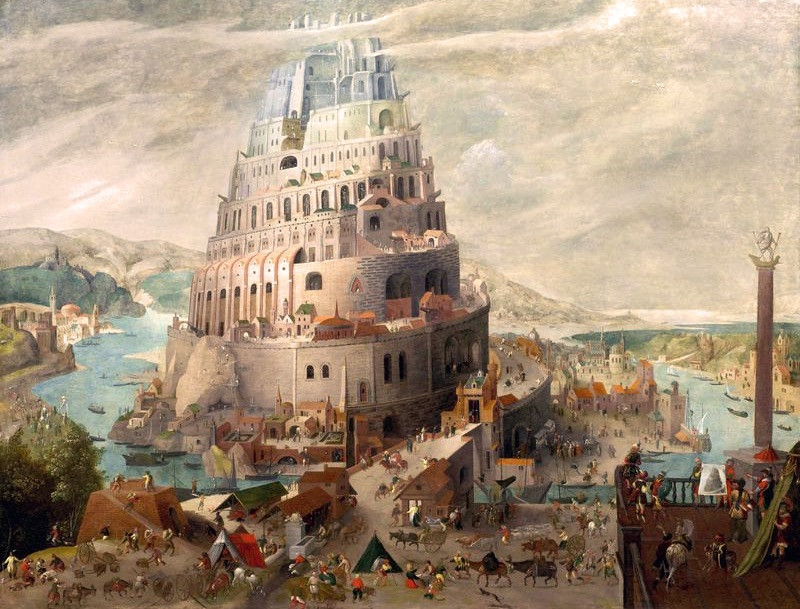
\includegraphics[width=.9\linewidth]{./tower-of-babel.jpg}
\end{center}
\end{block}
\end{frame}

\section{Imaginary Computing}
\label{sec:org5832048}
\begin{frame}[label={sec:org3a4cf92},fragile]{Imaginary Computing: Paracosm vs Metaverse}
 \begin{block}{Imaginary Web}
The imaginary web is a network of paracosms
and metaverses.

\begin{verbatim}
1  imaginary internet
2  imaginary web
3      An imaginary world-wide-web is an
4      analog of the World-Wide-Web imagined by a
5      language model.
\end{verbatim}
\end{block}

\begin{block}{emacs}
\begin{description}
\item[{Rich media}] In the World Wide Web of the 90s and 00s, \uline{rich media}
was considered to be large files including
images and music. In the 2010s, this has become
access to information behind a paywall and in
the 2020s, this will be access to \uline{intelligent}
and \uline{truthful} media.

\item \href{https://semiosis.github.io/looking-glass/}{Looking-Glass: An imaginary-web browser for emacs}
\item \href{https://mullikine.github.io/posts/the-imaginary-web-with-codex/}{Browsing the imaginary web}
\item \href{https://mullikine.github.io/posts/search-the-web-with-codex/}{Search the web/imaginary web without Google}
\item \href{https://mullikine.github.io/posts/alephalpha-for-alttext/}{Use AI to empower people to understand rich media}
\begin{itemize}
\item How to create a textual description of Rich Media
\end{itemize}
\end{description}
\end{block}
\end{frame}

\begin{frame}[label={sec:org7f3bd43}]{Paracosm vs Metaverse}
\begin{block}{Definitions}
\begin{itemize}
\item Paracosm
\begin{itemize}
\item Privacy
\item Personal truth
\item Freedom of imagination
\end{itemize}
\item Metaverse
\begin{itemize}
\item Getting cozy with Mark Zuckerberg's imaginarium, an intellectual prison
\end{itemize}
\end{itemize}
\end{block}
\end{frame}

\begin{frame}[label={sec:org21f488e}]{Philosophy}
\begin{block}{Simulacra and Science Fiction}
Jean Baudrillard speaks about the gap
between the real and the imaginary.

We no longer imagine a world radically
different from the real one, but
rather a world that's a mere expansion
of the real one.

In the postmodern society the gap
between the real and the imaginary
disappears completely, and we are no
longer capable of ideal projections
(of imagining new worlds).

We can only imagine mere
reconfigurations of our world, or
simply relive the ideal projections of
past times.
\end{block}
\end{frame}

\begin{frame}[label={sec:orgb76d799}]{Philosophy}
\begin{block}{Truth (epistemology and alethiology)}
The Future of Humanity Institute (Oxford)
seems to think this is an important topic.

\begin{itemize}
\item \href{https://arxiv.org/abs/2110.06674}{ 2110.06674  Truthful AI}
\item Datasets are a source of constructivist truth
\item Language models are snaphots of society, and a source of several types of truth
\begin{itemize}
\item \href{https://www.youtube.com/watch?v=kP-dXK9JEhY}{Symbolic Knowledge Distillation}
\end{itemize}
\item Blockchain is a source of consensus, a type of truth
\begin{itemize}
\item \url{https://mullikine.github.io/posts/language-models-as-truth/}
\end{itemize}
\end{itemize}
\end{block}
\end{frame}

\begin{frame}[label={sec:org377ea6b}]{Philosophy}
\begin{block}{Structuralism: Language based on sign relations}
What do these things have in common:
\begin{itemize}
\item Universal Grammar (UG) / Language Acquisition
\item C++ template metaprogramming
\item GPT-3
\end{itemize}

Knowledge exists at compile-time (DNA, preprocessor, training).
\end{block}
\end{frame}

\begin{frame}[label={sec:org96094a5}]{Philosophy}
\url{http://github.com/semiosis/glossaries-gh/blob/master/semiotics.txt}

\begin{block}{Structuralism: Language based on sign relations}
Structural linguistics / structuralism is the
theoretical position that finds meaning in the
relation between things, rather than in things
in isolation.

In other words, it gives primacy to pattern
over substance.

Such meanings may be either part of a
universal pattern or culturally determined.

Denotes schools or theories in which language
is conceived as a self-contained, self-
regulating semiotic system whose elements are
defined by their relationship to other
elements within the system.
\end{block}
\end{frame}

\section{Preliminaries}
\label{sec:org39cc8c5}
\subsection{GPT-3}
\label{sec:org779364d}
\begin{frame}[label={sec:org274bede},fragile]{Text Generator}
 \begin{block}{Background knowledge}
{\footnotesize
\begin{itemize}
\item \texttt{GPT-3} is a \texttt{seq2seq} model (a text generator)
\begin{itemize}
\item It's stochastic but can be configured to be deterministic.
\end{itemize}
\end{itemize}
}
\end{block}

\begin{block}{Key concepts}
{\footnotesize
\begin{itemize}
\item prompt,
\item completion, and
\item tokens
\end{itemize}
}
\end{block}

\begin{block}{Limitations}
{\footnotesize
Combined, the text prompt and generated
completion must be below 2048 tokens (roughly
\textasciitilde{}1500 words).

\begin{description}
\item[{context-stuffing}] With only 2048 tokens, you need to make
use of your real estate by providing
instructions and making implicit
information explicit.
\end{description}
}
\end{block}
\end{frame}

\subsection{A new programming paradigm}
\label{sec:orgfbd6146}
\begin{frame}[label={sec:org8e405e2},fragile]{Prompt Engineering}
 \begin{block}{Characteristics}
{\footnotesize
\begin{itemize}
\item declarative, like \texttt{html}
\item stochastic, like \texttt{problog}
\item Unlocks new types of applications
\item Speeds up development
\end{itemize}
}
\end{block}
\end{frame}

\begin{frame}[label={sec:org086e396},fragile]{Some prompts I've made}
 \begin{block}{\texttt{generate-vim-command.prompt}}
{\footnotesize
\begin{verbatim}
 1  Vim
 2  
 3  Insert "Q: " at the start of the line
 4  :%s/^/Q: /g.
 5  ###
 6  Remove whitespace from the start of each line
 7  :%s/^\s*/\1/g
 8  ###
 9  Join each line with the next line
10  :1,$j
11  ###
12  Make all occurrences of Steve lowercase
13  :%s/Steve/steve/g
14  ###
15  <1>
\end{verbatim}
}
\end{block}
\end{frame}

\begin{frame}[label={sec:org2f1ec3a}]{Tasks suitable for GPT-3}
\begin{block}{Classification}
\begin{itemize}
\item Tweet Sentiment
\item Company categorization
\item Labeling parts of speech
\end{itemize}

{\footnotesize
\begin{itemize}
\item \url{http://github.com/semiosis/prompts/blob/master/prompts/tweet-sentiment-classifier.prompt}
\item \url{http://github.com/semiosis/prompts/blob/master/prompts/keyword-extraction.prompt}
\end{itemize}
}
\end{block}
\end{frame}

\begin{frame}[label={sec:orga42e18f}]{Tasks suitable for GPT-3}
\begin{block}{Generation}
\begin{itemize}
\item Idea Generator
\end{itemize}

Come up with silly inventions.

\begin{center}
\includegraphics[width=.9\linewidth]{./silly-inventions.png}
\end{center}
\end{block}
\end{frame}

\begin{frame}[label={sec:org4f1465a}]{Tasks suitable for GPT-3}
\begin{block}{Conversation}
\begin{itemize}
\item Q\&A agent
\item Sarcastic chatbot
\end{itemize}

{\footnotesize
\url{http://github.com/semiosis/prompts/blob/master/prompts/sarcastic-response.prompt}
}
\end{block}
\end{frame}

\begin{frame}[label={sec:org45e9c32},fragile]{Design patterns}
 Taken from Prompt Design 101.

These are manual techniques which should be
encoded in a DSL when generating prompts.

\begin{block}{1. Reflective description of the task}
State what the prompt does at the start.

At the start of the example we state in plain
language what the classifier does:

\begin{verbatim}
1  This is a tweet sentiment classifier.
\end{verbatim}

By stating this up front, it helps the API
understand much more quickly what the goal of
the response is supposed to be and you’ll end
needing to provide fewer examples.
\end{block}
\end{frame}

\begin{frame}[label={sec:org3e646a6},fragile]{Design patterns}
 Taken from Prompt Design 101.

These are manual techniques which should be
encoded in a DSL when generating prompts.

\begin{block}{2. Use separators between examples}
Example: \texttt{\#\#\#}.

You can use other characters or line breaks,
but \texttt{\#\#\#} works pretty consistently and is
also an easy to use stop sequence.

Whatever separator you use, make sure that
it’s clear to the API where an example starts
and stops.
\end{block}
\end{frame}

\begin{frame}[label={sec:orge845bb0},fragile]{Design patterns}
 Taken from Prompt Design 101.

These are manual techniques which should be
encoded in a DSL when generating prompts.

\begin{block}{3. Mutiplexer Part 1}
Make a prompt more efficient / cheaper.

Design it to generate multiple results from
one API call.

{\tiny
\begin{verbatim}
 1  This is a tweet sentiment classifier
 2  Tweet: "I loved the new Batman movie!"
 3  Sentiment: Positive
 4  ###
 5  Tweet: "I hate it when my phone battery dies"
 6  Sentiment: Negative
 7  ###
 8  Tweet: "My day has been 👍"
 9  Sentiment: Positive
10  ###
11  Tweet: "This is the link to the article"
12  Sentiment: Neutral
13  ###
14  Tweet text
\end{verbatim}

}
\end{block}
\end{frame}

\begin{frame}[label={sec:org9448e95},fragile]{Design patterns}
 Taken from Prompt Design 101.

These are manual techniques which should be
encoded in a DSL when generating prompts.

\begin{block}{3. Mulitplexer Part 2}
{\tiny
\begin{verbatim}
 1  1. "I loved the new Batman movie!"
 2  2. "I hate it when my phone battery dies"
 3  3. "My day has been 👍"
 4  4. "This is the link to the article"
 5  5. "This new music video blew my mind"
 6  
 7  Tweet sentiment ratings:
 8  1: Positive
 9  2: Negative
10  3: Positive
11  4: Neutral
12  5: Positive
13  
14  ###
15  Tweet text
\end{verbatim}
}
\end{block}
\end{frame}

\begin{frame}[label={sec:orgee4cfec},fragile]{Design patterns}
 Taken from Prompt Design 101.

These are manual techniques which should be
encoded in a DSL when generating prompts.

\begin{block}{3. Multiplexer Part 3}
{\footnotesize
\begin{verbatim}
1  "I can't stand homework"
2  "This sucks. I'm bored 😠"
3  "I can't wait for Halloween!!!"
4  "My cat is adorable ❤️❤️"
5  "I hate chocolate"
6  Tweet sentiment ratings:
7  1.
\end{verbatim}
}
\end{block}
\end{frame}

\begin{frame}[label={sec:orgcd024b0}]{Techniques}
\begin{block}{Query Reformulation}
\url{https://www.sciencedirect.com/topics/computer-science/query-reformulation}

You can improve the quality of the responses
by making a longer more diverse list in your
prompt.

One way to do that is to start off with one
example, let the API generate more and select
the ones that you like best and add them to
the list.

A few more high-quality variations can
dramatically improve the quality of the
responses.
\end{block}
\end{frame}

\section{Explanations}
\label{sec:org8845086}
\subsection{Using \texttt{pen.el}}
\label{sec:orgeaf8f64}
\begin{frame}[label={sec:orgd14c461},fragile]{\texttt{pen.el}}
 \begin{block}{\texttt{pen.el}: Prompt Engineering in emacs}
{\footnotesize
\texttt{pen.el} facilitates the creation,
development, discovery and usage of prompts to
a Language Model such as GPT-3.

\begin{itemize}
\item Create elisp functions based on GPT-3 prompts
\item Chain GPT-3 queries together using keyboard macros and functions
\item Interactively query, generate and transfrom both prose and code
\item Use GPT-3 as a search engine within emacs
\end{itemize}
}
\end{block}
\end{frame}

\subsection{Using \texttt{pen.el}}
\label{sec:org514f05f}
\begin{frame}[label={sec:org3cbdf23},fragile]{\texttt{pen.el}}
 \begin{block}{\texttt{pen.el} modes Part 1}
{\footnotesize
\uline{\alert{Prompt-Engineering Minor Mode}}

\texttt{prompt-engineering-mode} is a global minor
mode for emacs that provides keybindings for
creating and executing prompts generally
across emacs.

\uline{\alert{Prompt Description Major Mode}}

\texttt{prompt-description-mode} is a major mode for
editing \texttt{.prompt} files.

The \texttt{.prompt} file format is based on YAML and
an associated schema, which defines the keys
which are expected.
}
\end{block}
\end{frame}

\subsection{Using \texttt{pen.el}}
\label{sec:org43c4ab3}
\begin{frame}[label={sec:org3964a4f},fragile]{\texttt{pen.el}}
 \begin{block}{\texttt{pen.el} modes Part 2}
{\footnotesize
\uline{\alert{Pen Messenger Minor Mode}}

\texttt{pen-messenger-mode} is a minor mode for
enhancing an emacs-based messenger client with
GPT-3 capabilities, such as emoji generation.

\uline{\alert{Pen Conversation Mode}}

\texttt{prompt-conversation-mode} is a major mode designed to facilitate
ongoing conversation with a prompt-based GPT-3 chatbot.

\uline{\alert{GPT-3 Training Mode}}

The goal of this mode is to facilitate the
workflow of training on OpenAI's API.
}
\end{block}
\end{frame}

\begin{frame}[label={sec:orgdabdca0},fragile]{Prompt YAML format Part 1}
 \begin{block}{\texttt{meeting-bullets-to-summary.prompt}}
\begin{verbatim}
 1  title: "meeting bullet points to summary"
 2  prompt: |+
 3      Convert my short hand into a first-hand
 4      account of the meeting:
 5  
 6      <1>
 7  
 8      Summary:
 9  engine: "davinci-instruct-beta"
10  temperature: 0.7
11  max-tokens: 60
\end{verbatim}
\end{block}
\end{frame}

\begin{frame}[label={sec:org5239f78},fragile]{Prompt YAML format Part 2}
 \begin{block}{\texttt{meeting-bullets-to-summary.prompt}}
\begin{verbatim}
1  top-p: 1
2  frequency-penalty: 0.0
3  presence-penalty: 0.0
4  best-of: 1
5  stop-sequences:
6  - "\n\n"
7  conversation-mode: no
8  stitch-max: 0
\end{verbatim}

\begin{description}
\item[{stitch-max}] Keep stitching together until reaching this limit.
This allows a full response for answers which may need n*max-tokens to reach the stop-sequence.
\end{description}
\end{block}
\end{frame}

\begin{frame}[label={sec:orgdeb6191},fragile]{Prompt YAML format: Part 3}
 \begin{block}{\texttt{meeting-bullets-to-summary.prompt}}
\begin{verbatim}
1  vars:
2  - "notes"
3  examples:
4  - |+
5      Tom: Profits up 50%
6      Jane: New servers are online
7      Kjel: Need more time to fix software
8      Jane: Happy to help
9      Parkman: Beta testing almost done
\end{verbatim}
\end{block}
\end{frame}

\section{\texttt{semiosis}}
\label{sec:org7c3fbbe}
\subsection{\texttt{pen.el}}
\label{sec:orge303b84}
\begin{frame}[label={sec:org22b3e83},fragile]{\texttt{Prompts as functions}}
 \begin{block}{\texttt{pen-generate-prompt-functions}}
Generate prompt functions for the files in the
prompts directory Function names are prefixed
with \texttt{pen-pf-} for easy searching.

\url{http://github.com/semiosis/prompts}
\end{block}
\end{frame}

\subsection{\texttt{examplary}}
\label{sec:org01f676d}
\begin{frame}[label={sec:orga16da5e},fragile]{\texttt{examplary}: examples as functions}
 An example-oriented DSL that can be used to
construct and compose NLP tasks.

Why is a DSL needed for this? Just to make the
code a little more terse.

\begin{block}{Regex}
\url{https://github.com/pemistahl/grex}

{\footnotesize
\begin{verbatim}
1  (def regex
2    "example 1\nexample2" "^example [12]$"
3    "example 2\nexample3" "^example [23]$"
4    "pi4\npi5" "^pi[45]$")
\end{verbatim}
}
\end{block}
\end{frame}

\begin{frame}[label={sec:org31feab3},fragile]{\texttt{examplary}: examples as functions}
 \begin{block}{Analogy}
{\footnotesize
\begin{verbatim}
 1  (def analogy
 2    ;; Each line is a training example.
 3    "NNs" "NNs are like genetic algorithms in
 4    that both are systems that learn from
 5    experience"
 6    "Social media" "Social media is like a
 7    market in that both are systems that
 8    coordinate the actions of many
 9    individuals.")
10  
11  (def field
12    "chemistry" "study of chemicals"
13    "biology" "study of living things")
\end{verbatim}
}
\end{block}
\end{frame}

\section{Demonstrations}
\label{sec:org192d4e1}
\begin{frame}[label={sec:org676f24e}]{Something funny}
\begin{block}{Vexate a simple instruction}
\begin{center}
\includegraphics[width=.9\linewidth]{./complicate.png}
\end{center}
\end{block}
\end{frame}

\begin{frame}[label={sec:org1b1b996}]{Something funny}
\begin{block}{How to crack an egg}
\begin{center}
\includegraphics[width=.9\linewidth]{./crack-an-egg.png}
\end{center}
\end{block}
\end{frame}

\begin{frame}[label={sec:orgeeef585}]{Create a prompt}
\begin{block}{Ask the audience}
\begin{itemize}
\item What type of text to generate
\begin{itemize}
\item Could be code, prose, etc.
\end{itemize}
\end{itemize}
\end{block}
\end{frame}

\section{Appendix}
\label{sec:org9149015}
\subsection{Additional reading}
\label{sec:orgfd9efef}
\begin{frame}[label={sec:orgd0b63c5}]{Tutorials}
\begin{block}{Ruby}
{\footnotesize
\url{https://www.twilio.com/blog/generating-cooking-recipes-openai-gpt3-ruby}
}
\end{block}
\end{frame}
\end{document}